\section{Calculation of the local energy}

At the sampling part we skipped over an important line.

\begin{minted}{python}
  E_local = local_energy_func(H, dist_s)
\end{minted}

Where we have to calculate the local energy of the quantum system in question. We know that the local energy of a particular sample state $\ket{s}$ can be calculated as

\begin{equation}
  E_{loc} = \displaystyle\frac{\bra{s}H\ket{\psi_{rbm}}}{\braket{s}{\psi_{rbm}}} \; ,
  \label{eq:local_imp}
\end{equation}

but here we will explain in more detail how this is done for the each of the different systems we are looking at. First of all it is important to remember the structure of the input to our function calculating the local energy. We want to vectorize the calculations as much as possible so the input will be all $m$ samples, taken with the Gibbs or Metropolis-Hastings algorithm, together in one array:

\begin{equation}
  \mathbf{S} = \left [ s_0, s_1, \dots, s_m \right] \; .
  \label{eq:Samples_set}
\end{equation}

To calculate the local energy for the Lipkin and Pairing model we need to have the wave function $\ket{\psi__{rbm}}$.

\begin{equation}
  \ket{\Psi_{rbm}} = \alpha_0\ket{\psi_0} + \alpha_1\ket{\psi_1} + \dots + \alpha_n\ket{\psi_n}
\end{equation}

The coefficients can be approximated. If we define $N_i$ as the number of state $\ket{\psi_i}$ in our sample set $\boldsymbol{S}$, then we have.

\begin{equation}
  \ket{\Psi_{rbm}} \approx \frac{N_0}{m}\ket{\psi_0} +\frac{N_1}{m}\ket{\psi_1} +\dots + \frac{N_n}{m}\ket{\psi_n}
\end{equation}

as an approximation of the machine state.

Looking at the different parts of $E_{loc}$ we have for a example state $\ket{b} \in \boldsymbol{S}$ that

\begin{equation}
  \braket{b}{\phi_{rbm}} = \alpha_i ,
\end{equation}

where $i$ would correspond to where the condition $\ket{b} = \ket{\phi_i}$ is fulfilled. To calculate the numerator of $E_{loc}$ we start with

\begin{equation}
  H\ket{\Psi_{rbm}} =  \alpha_0H\ket{\psi_0} + \alpha_1H\ket{\psi_1} + \dots + \alpha_nH\ket{\psi_n}
\end{equation}

The hamiltonian transforms the states into a new one

\begin{equation}
  H\ket{\psi_i} = \beta_{i,0}\ket{\psi_0} + \dots + \beta_{i,n}\ket{\psi_n}
\end{equation}

so we get

\begin{align}
  H\ket{\Psi_{rbm}} = \alpha_0  ( \beta_{0,0}\ket{\psi_0} &+ \dots + \beta_{0,n}\ket{\psi_n}  ) \\
 + \alpha_1  ( \beta_{1,0}\ket{\psi_0} &+ \dots + \beta_{1,n}\ket{\psi_n}  ) \\
&\vdots \\
+ \alpha_n  ( \beta_{n,0}\ket{\psi_0} &+ \dots + \beta_{n,n}\ket{\psi_n}  ) 
\end{align}

We then have that for the example state $\ket{b}$

\begin{equation}
  \bra{b}H\ket{\Psi_{rbm}} = \sum_{i=0}^n \alpha_j\beta_{i,j} \; ,
\end{equation}

where $j$ again is the corresponding state $\ket{b} = \ket{\psi_j}$.

In the practical calculations we will use the approximated coefficients. To do so we first we create an array of basis states.

\begin{minted}{python}
def create_basis(n, dtype, device):
    basis = torch.tensor(
        list(itertools.product([0, 1], repeat=n)),
        dtype = dtype,
        device= device
    )
    return basis
\end{minted}

where the \mintinline{python}{itertools.product(...)} creates all combinations of 0 and 1 into a array, and the rest is to make into a PyTorch tensor. With the basis in place we can check it against our samples.

\begin{minted}{python}
  
def amplitudes(samples, basis):
    weight = torch.sum(
      torch.all(samples[:, None] == basis, dim = -1), 
      dim=0
    )

    non_zero_mask = torch.where(weight!=0)
    weight[weight==0] = 1

    mask = torch.where(
      torch.all(samples[:, None] == basis, dim = -1)
    )[1]

    diff_basis = torch.sum(
        torch.logical_xor(basis[:, None], basis), dim=-1
    )

    return weight, non_zero_mask, mask, diff_basis
\end{minted}

The \mintinline{python}{weight} creates an array of where it has counted how many times each of the basis states appear in the sample set. \mintinline{python}{non_zero_mask} is to prevent division by zero when calculating the local energy when a basis state is not a part of the machine state. The \mintinline{python}{mask} is a tool to only needing to calculate the local energy for each basis state instead of each sample. We then use \mintinline{python}{mask} to extract the local energy of a sample from its matching basis state. Finally \mintinline{python}{diff_basis} checks how many particles excite up or de-excite down between each of the basis states. Using the broadcasting functionality.
\vspace{\baselineskip}
\\
\begin{*equation}
  \text{\mintinline{python}{xor}} \left (\begin{bmatrix}
      \ket{\psi_0} \\ \vdots \\ \ket{\psi_n} \end{bmatrix}, \; \left [\ket{\psi_0}, \dots , \ket{\psi_n}\right ] \right ) \rightarrow \begin{bmatrix}
  \text{\mintinline{python}{xor}} \left (\ket{\psi_0}, \ket{\psi_0} \right ) & \dots & \text{\mintinline{python}{xor}} \left (\ket{\psi_0}, \ket{\psi_n} \right ) \\
                                                                     \vdots   &  & \vdots \\
                                                                     \text{\mintinline{python}{xor}} \left (\ket{\psi_n}, \ket{\psi_0} \right ) & \dots & \text{\mintinline{python}{xor}} \left (\ket{\psi_n}, \ket{\psi_n} \right )
    \end{bmatrix}
\end{*equation}
\vspace{\baselineskip}
\\
We then have a approximation of our machine state $\ket{\psi}$ and the analysis of it to calculate the hamiltonian's effect on it. The next steps varies with the hamiltonian of the system.

\subsection{The Lipkin model} \label{section:imp_local}

The Lipkin model hamiltonian is defined as

\begin{equation} 
    H = \sum_{p\sigma} \left ( \frac{1}{2} \sigma \varepsilon \right ) \hc{a}{p\sigma}\op{a}{p\sigma} + \frac{V}{2}\sum_{pp'\sigma} \hc{a}{p\sigma} \hc{a}{p'\sigma} \op{a}{p'-\sigma}\op{a}{p-\sigma} + \frac{W}{2} \sum_{pp'\sigma} \hc{a}{p\sigma} \hc{a}{p'-\sigma} \op{a}{p'\sigma}\op{a}{p-\sigma} \; , 
\end{equation}

For a more structured explanation we separate the hamiltonian in three parts:

\begin{align}
  H_{\varepsilon} &= \sum_{p\sigma} \left ( \frac{1}{2} \sigma \varepsilon \right ) \hc{a}{p\sigma}\op{a}{p\sigma}\\ 
  H_V &= \frac{V}{2}\sum_{pp'\sigma} \hc{a}{p\sigma} \hc{a}{p'\sigma} \op{a}{p'-\sigma}\op{a}{p-\sigma}\\
  H_W &= \frac{W}{2} \sum_{pp'\sigma} \hc{a}{p\sigma} \hc{a}{p'-\sigma} \op{a}{p'\sigma}\op{a}{p-\sigma}  \; .
  \label{eq:LMG_split_H}
\end{align}

 A state $\ket{b}$ contributes for the different parts as follows:

\begin{itemize}
  \item $H_{\varepsilon}$ - the same state $\ket{b}$.
  \item $H_V$ - states that are a excited or de-excited pair away from the state $\ket{b}$.
  \item $H_W$ - states one excited or de-excited particle away from $\ket{b}$.
\end{itemize}

We separate the different parts then sum them together at the end.

\begin{minted}{python}

def lipkin_local(eps, V, W, samples, basis):
    weight, non_zero_weight, mask = amplitudes(samples, basis)
    non_zero = weight[non_zero_mask]
    non_zero_diff = diff_basis[non_zero_mask]

    N_0 = torch.sum(basis == 0, dim=-1)
    N_1 = torch.sum(basis == 1, dim=-1)
    
    H_0 = 0.5*eps*(N_1-N_0)
    H_eps = H_0[mask]

    H_1 = V*torch.sum(non_zero[:, None]*(non_zero_diff == 2), dim=0)/weight
    H_V = H_1[mask]
    
    H_2 = W*torch.sum(non_zero[:, None]*(non_zero_diff == 1), dim=0)/weight
    H_W = H_2[mask]
    
    E = (H_eps - H_V - H_W)
    return E

\end{minted}

For the $H_{\varepsilon}$ contribution we start of by calculating the number of particles in the first and second layer.

\begin{minted}{python}
    N_0 = torch.sum(basis == 0, dim=-1)
    N_1 = torch.sum(basis == 1, dim=-1)
\end{minted}

The particles in the first layer contribute with negative spin and the particles in the second layer contribute positively, so we get that.

\begin{minted}{python}
    H_0 = 0.5*eps*(N_1-N_0)
\end{minted}

We then have an array of the machine states amplitudes multiplied by $\varepsilon$. Applying \mintinline{python}{mask} to this array then selects the correct value for each sample without having to calculate duplicates more than once. We then have the $H_{\varepsilon}$ contribution for each sample directly:

\begin{minted}{python}
    H_eps = H_0[mask]
\end{minted}

We then calculate the difference between the basis states of the machine state, which is the states in \mintinline{python}{unique}, and the number of particles that change layer.

\begin{minted}{python}
    H_1 = 0.5*V*torch.sum(
      non_zero[:, None]*(non_zero_diff == 2), 
      dim=0
    )/weight
\end{minted}

Here it is important to notice that even if we only take the contribution of $H\ket{\psi_i}$ where $\ket{\psi_i} \in \ket{\psi_{rbm}}$ the transformed state can contain a basis state that is not a part of the machine state. Hence the removing of zero-valued amplitudes in the \mintinline{python}{weight} array is necessary. If we assume that the machine state contains every basis state for simplicity we have that:
\vspace{\baselineskip}
\\
\begin{equation*}
  \begin{gathered}
    \text{\mintinline{python}{ non_zero[:, None]*(non_zero_diff == 2)}} \rightarrow \boldsymbol{M}_{diff, 2} \\
    \\
    \boldsymbol{M}_{diff, 2} = \begin{bmatrix}
      N_0 \text{\mintinline{python}{xor}} \left (\ket{\psi_0}, \ket{\psi_0} \right ) & \dots & N_0  \text{\mintinline{python}{xor}} \left (\ket{\psi_0}, \ket{\psi_n} \right ) \\
      \vdots & & \vdots \\
      N_n  \text{\mintinline{python}{xor}} \left (\ket{\psi_n}, \ket{\psi_0} \right ) & \dots & N_n  \text{\mintinline{python}{xor}} \left (\ket{\psi_n}, \ket{\psi_n} \right )
    \end{bmatrix}
  \end{gathered}
\end{equation*}
\vspace{\baselineskip}
\\
And we have that $\bra{b}H\ket{\Psi_{rbm}} = \sum_{i=0}^n \alpha_j\beta_{i,j}$, so we add the rows together, which is the first dimension in python. We then divide by each of the basis states amplitude before transformation by the hamiltonian. The \mintinline{python}{mask} is then applied:

\begin{minted}{python}
    H_V = H_1[mask]
\end{minted}

For $H_W$ we have the exact same approach, only changing the condition of number of excited or de-excited particles to $1$:

\begin{minted}{python}
    H_2 = 0.5*W*torch.sum(
      non_zero[:, None]*(non_zero_diff == 1),
      dim=0
    )/weight
    H_W = H_2[mask]
\end{minted}

And lastly we subtract all the parts as defined in the full Lipkin hamiltonian:

\begin{minted}{python}
    E = (H_eps - H_V - H_W)
    return E
\end{minted}

which we return as an array of the local energy of each of the input samples. The Lipkin hamiltonian is costructed using the quasi spin matrices, and as such has a size of $n/2 + 1$ for an $n$-particle system. We will need to convert our basis into the new one by the states total spin $m$:

\begin{minted}{python}
def lipkin_amps(samples):
    size, n = samples.shape
    basis_m = torch.arange(-n, n+1, 2, dtype=samples.dtype, device=samples.device)
    samples_m = torch.sum(2*samples-1, dim=-1)
    weight = torch.sum(samples_m[:, None] == basis_m, dim=0)
    weight = weight/size
    weight = torch.sqrt(weight)
    non_zero_mask = torch.where(weight>0)
    weight[weight==0] = np.sqrt(1/size)
    mask = torch.where(samples_m[:, None] == basis_m)[1]
    
    return weight, non_zero_mask, mask
\end{minted}

where the \mintinline{python}{samples_m} is mathced excatly so.

\subsection{The Ising model}

For the Ising model we can calculate the local energy directly with:

\begin{equation}
  H(\boldsymbol{\sigma}) = J\sum_{<i,j>}\sigma^z_i\sigma^z_j + L \sum_i \sigma^x_i \; ,
  \label{eq:imp_hamil_ising}
\end{equation}

where $J$ is the interaction strength between nearest neighbors, and $L$ is the single particle energy against an external field. To calculate the coupling efficiently we take the whole set and shift it:

\begin{minted}{python}
def ising_1d_coupling(J, samples):
  pm = 2*samples - 1
  shift_r = torch.roll(pm, 1, 1)
  H_J = J*torch.sum(pm*shift_r, dim=-1)
  return H_J
\end{minted}

where we then assume the boundary conditions:

\begin{equation}
  \begin{gather}
  \mathbf{\sigma} = \begin{bmatrix} \sigma_0 & \sigma_1 & \dots & \sigma_{N-1}\end{bmatrix} \\
  \sigma_0 = \sigma_N \; ,
  \label{eq:ising_boundary_imp}
\end{gather}
\end{equation}

as explained in \ref{sec:ising_theory}. As the coupling part is inbound of each state, the $\sigma^z$ Pauli matrix rotates the state around the z-axis so it doesn't flip states, it creates only contributions the same state as itself.

\begin{minted}{python}
def ising_local(N, M, J, L, samples, basis_set):
    
    basis, diff_basis, H_J = basis_set
    weight, non_zero_mask, mask = amplitudes(samples, basis)
  
    H_s = torch.zeros_like(H_J)
    H_s[non_zero_mask] = H_J[non_zero_mask]

    non_zero = weight[non_zero_mask]
    non_zero_diff = diff_basis[non_zero_mask]
    H_L = L*torch.sum(non_zero[:, None]*(non_zero_diff==1), dim=0)/weight
    
    H = H_s + H_L
    return H[mask], torch.var(H)
\end{minted}

Where we have that $H_J$ is passed to the right ising coupling function depending on if its one or two dimensions:

\begin{minted}{python}
def ising_basis_set(N, M, J, L, basis_set):
    basis, diff_basis = basis_set
    if M == 1:
        H_J = ising_1d_coupling(J, basis)
    else:
        H_J = ising_2d_coupling(N, M, J, basis)
    return basis, diff_basis, H_J
\end{minted}

We then take out the states that aren't in the machine state by:

\begin{minted}{python}
    H_s = torch.zeros_like(H_J)
    H_s[non_zero_mask] = H_J[non_zero_mask]
\end{minted}

The field part of the Hamiltonian is essentially a spin flip, so states one spin different from eachother contributes. After selecting the parts of the \mintinline{python}{diff_basis} and \mintinline{python}{weights} that are a part of the machine state we do as with the Lipkin model and sum up each contribution:

\begin{minted}{python}
  H_L = L*torch.sum(non_zero[:, None]*(non_zero_diff==1), dim=0)/weight
\end{minted}

Finally we sum it together and use the mask to select the correct states.

\begin{minted}{python}
    H = H_s + H_L
    return H[mask], torch.var(H)
\end{minted}

The Ising model becomes drastically more interesting in higher dimensions, and we will look at the 2-dimensional Ising as well. We just expand our approach of shifting the input array. Practically the input will be a flattened array of the 2-dimensional grid.

\begin{minted}{python}
def ising_2d_coupling(N, M, J, samples):
    
    pm = 2*samples - 1
    pm = torch.reshape(pm, (pm.shape[0], M, N))
    up = torch.roll(pm, 1, 1)
    right = torch.roll(pm, 1, 2)
    H_J = up*pm + right*pm
    H_J = torch.sum(H_J, dim=-1)
    H_J = torch.sum(H_J, dim=-1)
    return H_J
\end{minted}

The closest neighbours in a grid is on both sides on the same row, and up and down on the column, but to not count pairs twice we only need to roll once in each direction. Reshaping the input we can use the \mintinline{python}{torch.roll(...)} function to shift the matrix in each of these directions, and then multiply and sum them together.

\subsection{The Heisenberg model}

The Heisenberg model's difference to the Ising model is the input, we go from binary spin to continuous, so we reuse the Ising model Hamiltonian for both one and two dimensions with only slight changes:

\begin{minted}{python}
def heisen_hamiltonian(N, M, J, L):
    import netket.hilbert as hb
    from netket.operator.spin import sigmax, sigmay, sigmaz

    hi = hb.Spin(s=1/2, N=N*M)
    H = sum([(L+0j)*sigmax(hi,i) for i in range(N)])
    if M == 1:
        for i in range(N):
            H += (J+0j)*sigmax(hi, i)*sigmax(hi, i)
            H += (J+0j)*sigmay(hi, i)*sigmay(hi, i)
            H += (J+0j)*sigmaz(hi, i)*sigmaz(hi, i)
    else:
        for _ in range(M):
            for i in range(N):
                H += (J+0j)*sigmax(hi, N*i)*sigmax(hi, (N*i+1)%N)
                H += (J+0j)*sigmax(hi, N*i)*sigmax(hi, (N*i+N)%(N*M))
                H += (J+0j)*sigmay(hi, N*i)*sigmay(hi, (N*i+1)%N)
                H += (J+0j)*sigmay(hi, N*i)*sigmay(hi, (N*i+N)%(N*M))
                H += (J+0j)*sigmaz(hi, N*i)*sigmaz(hi, (N*i+1)%N)
                H += (J+0j)*sigmaz(hi, N*i)*sigmaz(hi, (N*i+N)%(N*M))
    return np.array(H.to_dense().real)
\end{minted}

For each of the Pauli spin matrices we do the same as we did for $\sigma^z$ in the Ising Hamiltonian, though we here have to add $(J+0j)$ to make sure the matrix is initialized as complex valued. The Pauli-y matrix is complex valued, and we cannot add a float valued matrix and complex valued matrix together.

\subsection{The Pairing model}

 The Pairing model hamiltonian can be written as

\begin{equation}
  \hat{H} = \epsilon \sum_{p\sigma} \left(p-1\right)\hc{a}{p\sigma}\op{a}{p\sigma} - \frac{1}{2}g\sum_{pq}\hat{P}_p^+\hat{P}_q^-
  \label{eq:Pairing_model_imp}
\end{equation}

Where we have that

\begin{equation*}
  \begin{gathered}
    \hat{P}_p^+ = \hc{a}{p+}\hc{a}{p-}\\
    \hat{P}_p^- = \op{a}{p-}\op{a}{p+}
  \end{gathered}
\end{equation*}

First of we need to define how we will represent the states in the RBM's visual layer. In contrast to the Lipkin model, here we always have pairs moving together, so what we will do is have a $1$ in the visual layer represent one such pair. An example state

$$\ket{b} = \left[\;1, 0, 1, 0 \; \right]^T \; ,$$

would visually look like:

\vspace{\baselineskip}
\\
\begin{figure}[H]
  \begin{center}
    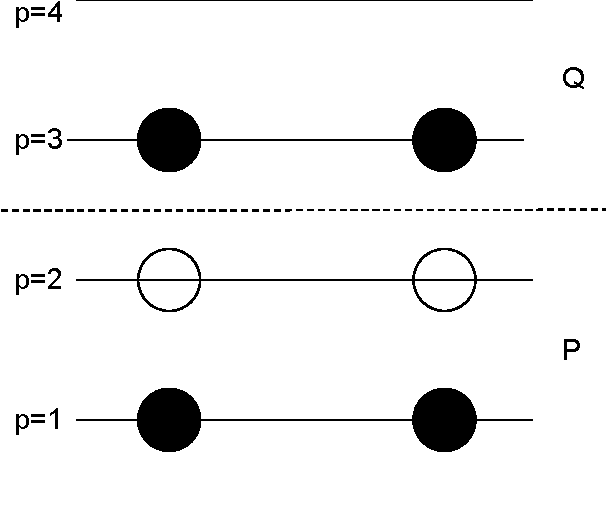
\includegraphics[width=0.5\textwidth]{Figures/Drawn/Pairing/pairing_imp_exp.pdf}
  \end{center}
\end{figure}

The Hamiltonian neither creates or destroys particles, so many states in our basis cannot be a part of the wavefunction, so we the Hamiltonian elements is set to zero. 

\begin{minted}{python}
def pairing_hamiltonian(basis, P, n, eps, g):

    mask_non = torch.where(torch.sum(basis, dim=-1) != n)[0]
    where = torch.where(basis==1)
    B_0 = torch.zeros_like(basis[:, 0])
    for i, a_one in enumerate(where[0]):
        B_0[a_one] += where[1][i]

    diff = torch.sum(
        torch.logical_xor(basis[:, None], basis),
        dim=-1
    )
    B_1 = 0.5*g*(diff==2)
    H = torch.diagflat(B_0) + B_1
    for i in mask_non:
        H[:, i] = 0
        H[i, :] = 0

    return np.array(H.cpu())
  \end{minted}

  We first check each state for the correct number of particles, or pairs in this case, and sum up the single particle energies for those states. We then check for a excited pair, which here would mean a difference of two since it is first removed from the first state and then created in the other. At last we zero out each row and column corresponding to an illegal state.


To consturct the Pairing Hamiltonian matrix we will will use a different approach to that of what we did with the Lipkin model, and we will explain in it more practically in the implementation section \ref{sec:pairing_imp}. Constricting our scope to where there are no split pairs we can represent the layers as particles in and of themselves instead. Our compuational basis here will the standard basis, where $\ket{0}$ indicates an empty layer $p$ and $\ket{1}$ indicates that the layer is occupied by a pair of fermions, a spin up and spin down. This then means we can the su over the spin in the hamiltonian, and we write it as:

$$\hat{H} = 2\epsilon \sum_p \left (p - 1 \right) \hc{a}{p}\op{a}{p} - \frac{1}{2}g \sum_{pq}\hc{a}{p}\op{a}{q} \; $$

We will start of with the concret example of a two-particle system with the layer truncation happening at $p=2$. We then have the standard basis $\ket{00}$, $\ket{10}$, $\ket{01}$, $\ket{11}$. The Hamiltonian matrix can be written as:

$$\mathbf{H} = \begin{bmatrix}
\bra{00} H \ket{00} & \bra{00} H \ket{10} &\bra{00} H \ket{01} & \bra{00} H \ket{11} \\
\bra{10} H \ket{00} & \bra{10} H \ket{10} &\bra{10} H \ket{01} & \bra{10} H \ket{11} \\
\bra{01} H \ket{00} & \bra{01} H \ket{10} &\bra{01} H \ket{01} & \bra{01} H \ket{11} \\
\bra{11} H \ket{00} & \bra{11} H \ket{10} &\bra{11} H \ket{01} & \bra{11} H \ket{11} \\
\end{bmatrix} \; ,
$$

The states $\ket{00}$ and $\ket{11}$ cannot be created through our Hamiltonian \ref{eq:Pairing_model_final} because we can only move pairs, not create or destroy them, so we can safely say that 

$$ H \ket{00} = H\ket{11} = 0$$

And that

where $\bra{s}$ and $\ket{s}$ are any other basis state. We then have only the block of four in the middle, and starting with $\bra{10}H\ket{10}$ we have that since no pairs are excited from $\ket{10} \rightarrow \ket{10}$, only the single particle energies contribute to this element of the Hamiltonian. We then only need to look at:

\begin{align*}
 &\; \; 2\varepsilon\bra{10}  \left (1 - 1 \right) \hc{a}{1}\op{a}{1} + \left (2 - 1 \right) \hc{a}{2}\op{a}{2} \ket{10} \\
 &= \bra{10} \hc{a}{2}\op{a}{2} \ket{10} \\
 &= 0
 \; ,
\end{align*}

and

\begin{align*}
 &\; \; 2\varepsilon\bra{01}  \left (1 - 1 \right) \hc{a}{1}\op{a}{1} + \left (2 - 1 \right) \hc{a}{2}\op{a}{2} \ket{01} \\
 &= \bra{01} \hc{a}{2}\op{a}{2} \ket{01} \\
 &= 2\varepsilon
 \; ,
\end{align*}

where $\bra{\alpha} \hc{a}{l}\op{a}{l} \ket{\beta} = 1$ when we have a pair in layer $l$ in both $\ket{\alpha}$ and $\ket{\beta}$, and becomes zero otherwise. 

To show that we can block-diagonalize the full Hamiltonian we will calculate the commutative relations between $\hat{H}_0$ and $\hat{V}$ with the spin projection $\hat{S}_z$ and the total spin $\hat{S}^2$. Starting with $\hat{S}_z$ given by:

\begin{equation}
  \hat{S}_z = \frac{1}{2}\sum_{pq} \sigma \hc{a}{pq}\op{a}{pq}\; .
  \label{eq:s_z}
\end{equation}

Further we have that

\begin{equation}
  \hat{S}^2 = \hat{S}_z^2 + \frac{1}{2} \left(\hat{S}_+\hat{S}_- + \hat{S}_-\hat{S}_+\right) \; ,
  \label{eq:s_2}
\end{equation}

where

\begin{equation}
  \hat{S}_{\pm} = \sum_p \hc{a}{p\pm}\op{a}{p\mp} \; . 
  \label{eq:s_pm}
\end{equation}

And the commutation relation
